% Figure 1: hero schematic. Pre-rendered to PDF (AAAI forbids pgfplots in the paper source; TikZ is kept out of it too).
% Layout: source prompt -> one hidden state -> three readers -> real outputs (rows = readers, columns = items).
% All strings are copied verbatim from result files, ALL AT LAYER 32 of the 14B:
%   our item curated:country_of_capital:28f48dbd (kept from the first draft; not selected for the size of any failure):
%     token-lens ranks of " North" / " Korea": runs/w2B_x5_14b/results.json L32 (raw J-lens 13 / 3, logit lens 5 / 2) and
%     runs/p2_B_14b/results.json L32 (cosine J-lens 10 / 3); the logit-lens top-5 there is a Chinese form of Korea,
%     " Korea", a Vietnamese form, " DPR", " North".
%     copy prompt: runs/w3_B_x3i3_14b_ans_L32/results.json (identity3:replace 0/8 " North America -> ..."; :t4 6/8);
%     continuation: runs/w4_B_x3cont_14b_ans_L32/results.json (continuation:replace:t4, 8/8 start with " North Korea").
%   bench item brh-ent-chem-wintergreen-ester: runs/w4_e1_14b_basic_cl/readouts/{jlens,x3c_t4}/basic_readout_mt.jsonl and
%     runs/w4_e2_14b_basic/readouts/x3_identity3_t4 (layer 32).
% Every piece of text is \small (9 pt at the 10 pt base) or larger, the AAAI in-figure minimum, at the 7.0 in print width.
\documentclass[10pt,border=2pt]{standalone}
\usepackage{newtxtext}
\usepackage[T1]{fontenc}
\usepackage{tikz}
\usetikzlibrary{arrows.meta,positioning,calc}
\definecolor{wblue}{HTML}{0072B2}
\definecolor{worange}{HTML}{E69F00}
\definecolor{wgreen}{HTML}{009E73}
\definecolor{wgray}{HTML}{555555}
\begin{document}
\small
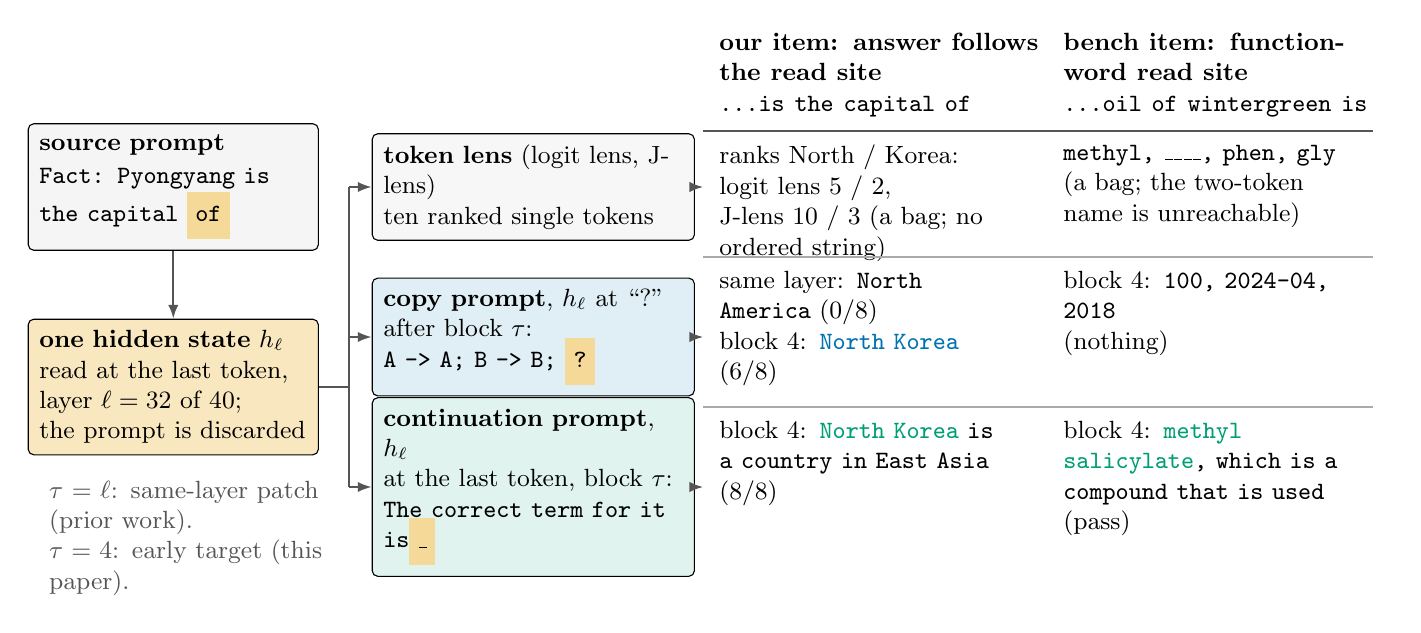
\begin{tikzpicture}[
  x=1in,y=1in,
  box/.style={draw,rounded corners=2pt,inner sep=4pt,align=left,font=\small},
  reader/.style={box,text width=1.50in,minimum height=0.50in},
  arr/.style={-{Latex[length=5pt]},thick,wgray},
  cell/.style={font=\small,align=left,inner sep=2pt,anchor=north west,text width=1.50in},
  hdr/.style={font=\small\bfseries,align=left,inner sep=2pt,anchor=south west,text width=1.62in}]

% ---------- column 1: source prompt and the one hidden state ----------
\node[box,fill=black!4,text width=1.34in] (src) at (0.72,1.78)
  {\textbf{source prompt}\\[1pt]\ttfamily Fact: Pyongyang is\\the capital \colorbox{worange!40}{\strut of}};
\node[box,fill=worange!25,text width=1.34in] (h) at (0.72,0.78)
  {\textbf{one hidden state} $h_\ell$\\ read at the last token,\\ layer $\ell=32$ of 40;\\ the prompt is discarded};
\draw[arr] (src) -- (h);

% ---------- column 2: three readers, one per row ----------
\node[reader,fill=black!3]  (r1) at (2.52,1.78) {\textbf{token lens} (logit lens, J-lens)\\ ten ranked single tokens};
\node[reader,fill=wblue!12] (r2) at (2.52,1.03) {\textbf{copy prompt}, $h_\ell$ at ``?''\\ after block $\tau$:\\ {\ttfamily A -> A; B -> B; \colorbox{worange!40}{\strut ?}}};
\node[reader,fill=wgreen!12] (r3) at (2.52,0.28) {\textbf{continuation prompt}, $h_\ell$\\ at the last token, block $\tau$:\\ {\ttfamily The correct term for it is\colorbox{worange!40}{\strut \_}}};
% bus from h to the three readers
\coordinate (bus) at (1.60,0.78);
\draw[wgray,thick] (h.east) -- (bus);
\draw[wgray,thick] (bus) -- (1.60,1.78);
\draw[wgray,thick] (bus) -- (1.60,0.28);
\draw[arr] (1.60,1.78) -- (r1.west);
\draw[arr] (1.60,1.03) -- (r2.west);
\draw[arr] (1.60,0.28) -- (r3.west);
% note on tau, under the hidden-state box, clear of every box
\node[font=\small,wgray,align=left,anchor=north west,text width=1.40in] at (0.05,0.36)
  {$\tau=\ell$: same-layer patch (prior work).\\ $\tau=4$: early target (this paper).};

% ---------- columns 3-4: real Qwen3-14B outputs, all at l = 32 ----------
\begin{scope}[shift={(3.42,0)}]
\node[hdr] (c1) at (0.00,2.10) {\textbf{our item}: answer follows the read site\\ {\ttfamily ...is the capital of}};
\node[hdr] (c2) at (1.72,2.10) {\textbf{bench item}: function-word read site\\ {\ttfamily ...oil of wintergreen is}};
\draw[wgray] (-0.05,2.06) -- (3.30,2.06);
% row 1: token lens (ranks of " North" / " Korea" at layer 32)
\node[cell] at (0.00,2.02) {ranks North / Korea: logit lens 5 / 2,\\ J-lens 10 / 3 (a bag; no ordered string)};
\node[cell] at (1.72,2.02) {{\ttfamily methyl, \_\_\_\_, phen, gly}\\ (a bag; the two-token name is unreachable)};
\draw[wgray!50] (-0.05,1.43) -- (3.30,1.43);
% row 2: copy prompt
\node[cell] at (0.00,1.39) {same layer: {\ttfamily North America} (0/8)\\ block 4: {\ttfamily\textcolor{wblue}{North Korea}} (6/8)};
\node[cell] at (1.72,1.39) {block 4: {\ttfamily 100, 2024-04, 2018}\\ (nothing)};
\draw[wgray!50] (-0.05,0.68) -- (3.30,0.68);
% row 3: continuation prompt
\node[cell] at (0.00,0.64) {block 4: {\ttfamily\textcolor{wgreen}{North Korea} is a country in East Asia} (8/8)};
\node[cell] at (1.72,0.64) {block 4: {\ttfamily\textcolor{wgreen}{methyl salicylate}, which is a compound that is used} (pass)};
\end{scope}
% arrows from each reader into its output row
\draw[arr] (r1.east) -- (3.37,1.78);
\draw[arr] (r2.east) -- (3.37,1.03);
\draw[arr] (r3.east) -- (3.37,0.28);
\end{tikzpicture}
\end{document}
